% This is samplepaper.tex, a sample chapter demonstrating the
% LLNCS macro package for Springer Computer Science proceedings;
% Version 2.20 of 2017/10/04
%
\documentclass[runningheads]{llncs}
%
\usepackage{amsmath}
\usepackage{booktabs} % For pretty tables
\usepackage{caption} % For caption spacing
\usepackage{subcaption} % For sub-figures
\usepackage{graphicx}
\usepackage{pgfplots}
\usepackage[all]{nowidow}
\usepackage[utf8]{inputenc}
\usepackage{tikz}
\usetikzlibrary{er,positioning,bayesnet}
\usepackage{multicol}
\usepackage{algpseudocode,algorithm,algorithmicx}
\usepackage{minted}
\usepackage{hyperref}
\usepackage[inline]{enumitem} % Horizontal lists

%\usepackage{natbib}
%\usepackage[style=authoryear]{biblatex}

% Used for displaying a sample figure. If possible, figure files should
% be included in EPS format.
%
% If you use the hyperref package, please uncomment the following line
% to display URLs in blue roman font according to Springer's eBook style:
% \renewcommand\UrlFont{\color{blue}\rmfamily}

\newcommand{\card}[1]{\left\vert{#1}\right\vert}
\newcommand*\Let[2]{\State #1 $\gets$ #2}
\definecolor{blue}{HTML}{1F77B4}
\definecolor{orange}{HTML}{FF7F0E}
\definecolor{green}{HTML}{2CA02C}

\pgfplotsset{compat=1.14}

\renewcommand{\topfraction}{0.85}
\renewcommand{\bottomfraction}{0.85}
\renewcommand{\textfraction}{0.15}
\renewcommand{\floatpagefraction}{0.8}
\renewcommand{\textfraction}{0.1}
\setlength{\floatsep}{3pt plus 1pt minus 1pt}
\setlength{\textfloatsep}{3pt plus 1pt minus 1pt}
\setlength{\intextsep}{3pt plus 1pt minus 1pt}
\setlength{\abovecaptionskip}{2pt plus 1pt minus 1pt}

\usepackage{Sweave}
\begin{document}
\Sconcordance{concordance:draft_v3.tex:draft_v3.Rnw:1 50 1 1 0 161 1}

%
\title{Residential Segregation in Brazil: An Inference Framework Based study for Selected Cities}
%
%\titlerunning{Abbreviated paper title}
% If the paper title is too long for the running head, you can set
% an abbreviated paper title here
%
\author{Renan Xavier Cortes\inst{1}}

%
%\authorrunning{F. Author et al.}
% First names are abbreviated in the running head.
% If there are more than two authors, 'et al.' is used.
%
\institute{Federal University of Rio Grande do Sul \\
\email{renan.cortes@ufrgs.br}\\}
%
\maketitle              % typeset the header of the contribution
%
\begin{abstract}
This is the abstract

\keywords{Residential Segregation \and Inference Framework \and Brazilian Cities \and PySAL}
\end{abstract}
%
%
%
\section{Introduction}\label{sec:introduction}

Residential segregation is a major topic of study

\cite{massey1988dimensions} goes here \cite{allen2015more}

Talk about it is census tract level (and not neighborhood)


\section{Related work}\label{sec:related-work}

\cite{cortes2020open}

Here, in this section I cite renan, \cite{rey2021comparative}

I also cite all brazilian papers of the literature
\cite{sousa2023nacional}
\cite{deSousaFilho2022nationwide}
\cite{barber2018cardioelsa}
\cite{barros2018unevengeographies}
\cite{barros2024saopaulolondres}
\cite{strauch2026bh20102022}
\cite{danilofranca2022fortaleza}

Why we chose those cities

\section{Framework} \label{subsec:statistical-summaries}

Here, I discuss the hyphotesis present the null hyphothesis and alternative hypothesis

and limitaitons of the approach recovering the Reviewer comments.

Discuss the dimensions o Massey...

Queen matrix

Segreagation measures choses

\section{Results}\label{subsec:statistical-summaries}

Hardware, 

\subsection{Point Estimation of segregation measures}\label{sec:sampling}


Here I put the maps
Here I put all point measurements and discuss



\begin{figure}[htbp]
    \centering
    
    \begin{subfigure}{0.48\textwidth}
        \centering
        \includegraphics[width=\linewidth]{figures/seg_profile_4314902.png}
        \caption{Porto Alegre, RS}
        \label{fig:1}
    \end{subfigure}
    \hfill
    \begin{subfigure}{0.48\textwidth}
        \centering
        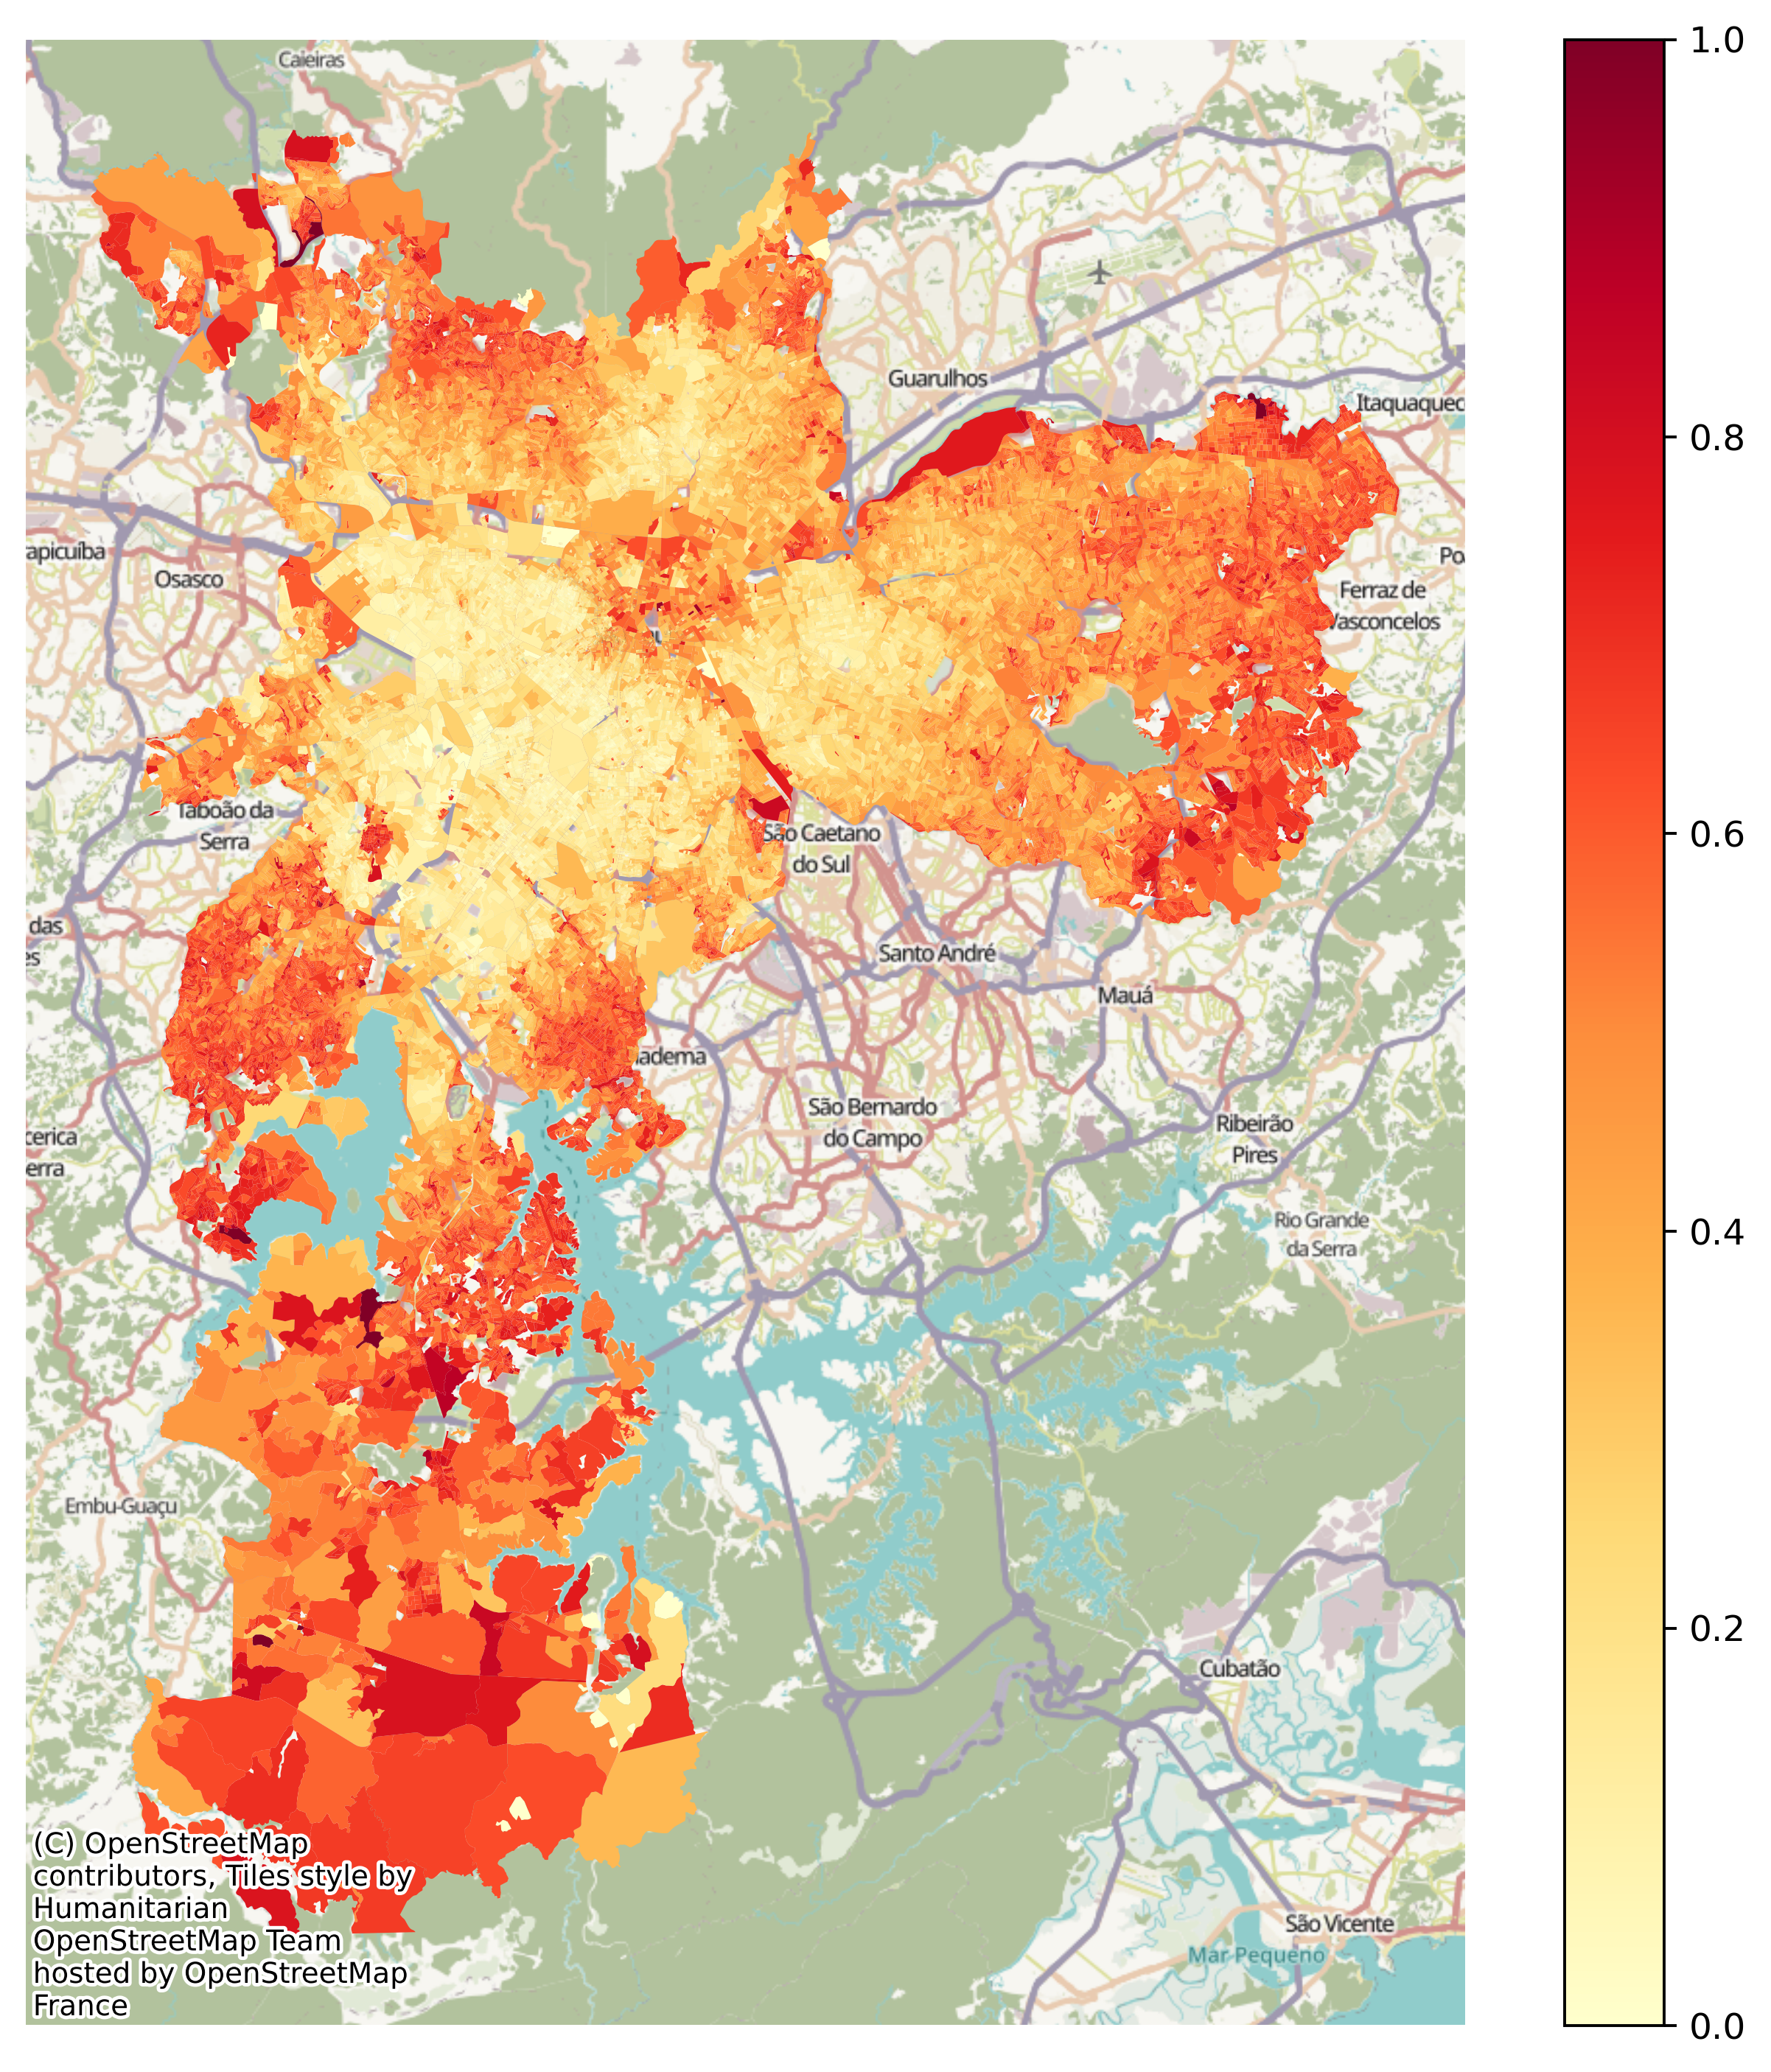
\includegraphics[width=\linewidth]{figures/seg_profile_3550308.png}
        \caption{São Paulo, SP}
        \label{fig:2}
    \end{subfigure}
    
    \vspace{0.5cm}
    
    \begin{subfigure}{0.48\textwidth}
        \centering
        \includegraphics[width=\linewidth]{figures/seg_profile_3304557.png}
        \caption{Rio de Janeiro, RJ}
        \label{fig:3}
    \end{subfigure}
    \hfill
    \begin{subfigure}{0.48\textwidth}
        \centering
        \includegraphics[width=\linewidth]{figures/seg_profile_3106200.png}
        \caption{Belo Horizonte, MG}
        \label{fig:4}
    \end{subfigure}
    
    \caption{Composition of all selected cities}
    \label{fig:2x2grid}
\end{figure}

\subsection{Inference results}\label{sec:sampling}

Computational challenges

\begin{figure}[H]
    \centering
    \includegraphics[width=0.5\textwidth]{figures/grid_plot_4314902_systematic.png}
    \caption{Point Estimation with systematic approach}
    \label{fig:grid_plot_4314902_systematic}
\end{figure}

\begin{figure}[H]
    \centering
    \includegraphics[width=0.5\textwidth]{figures/grid_plot_4314902_evenness.png}
    \caption{Point Estimation with evenness approach}
    \label{fig:grid_plot_4314902_evenness}
\end{figure}

\begin{figure}[H]
    \centering
    \includegraphics[width=0.5\textwidth]{figures/grid_plot_4314902_geographic_permutation.png}
    \caption{Point Estimation with Geographic Permutation approach}
    \label{fig:grid_plot_4314902_geographic_permutation}
\end{figure}


\section{Discussion and Future Work}\label{sec:statistical-summaries}


More cities
Comparative framework detangling with shapley
Street network based



%
% ---- Bibliography ----
%
% BibTeX users should specify bibliography style 'splncs04'.
% References will then be sorted and formatted in the correct style.
%
\bibliographystyle{splncs04}
%\bibliographystyle{plain}  % or another style
\bibliography{references}
%
\end{document}
